\begin{figure}[t]
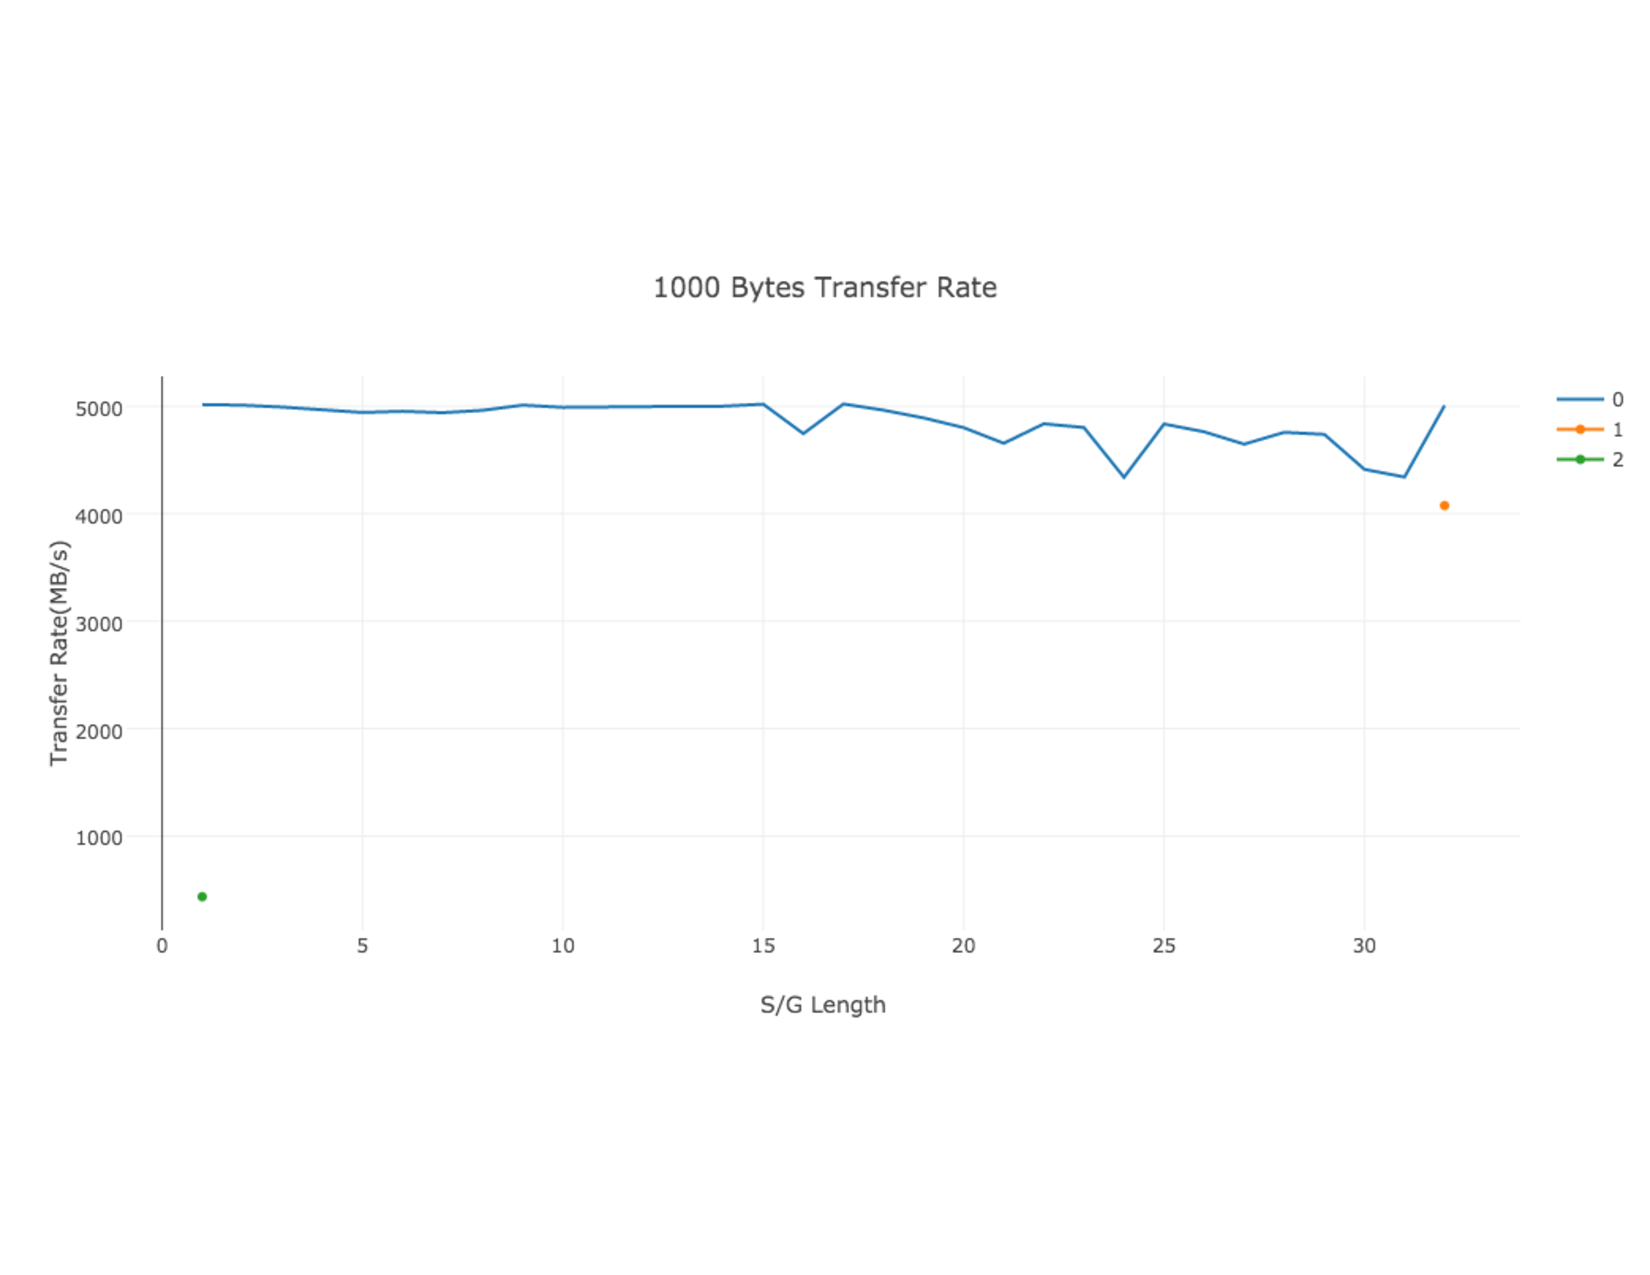
\includegraphics[width=\textwidth]{1000B_transrate.pdf}
\caption{Transmission rate for 100 B records over different RDMA verbs and 
various lengths of the scatter gather employed.
The green dot shows the performance for RDMA reads which is also unfair
since RDMA reads can only transmit a single record at a time. The yellow dot
shows RDMA write performance. The modes shown was an enum of the format 
\cpp{enum Mode \{ MODE_SEND, MODE_WRITE, MODE_READ\}}
\cpp{<infiniband/verbs.h> supports the various modes}
}
\label{fig:1000B_transrate}
\end{figure}
